\section{Introduction}
\label{sec:intro}

\begin{figure}[t]
\centering
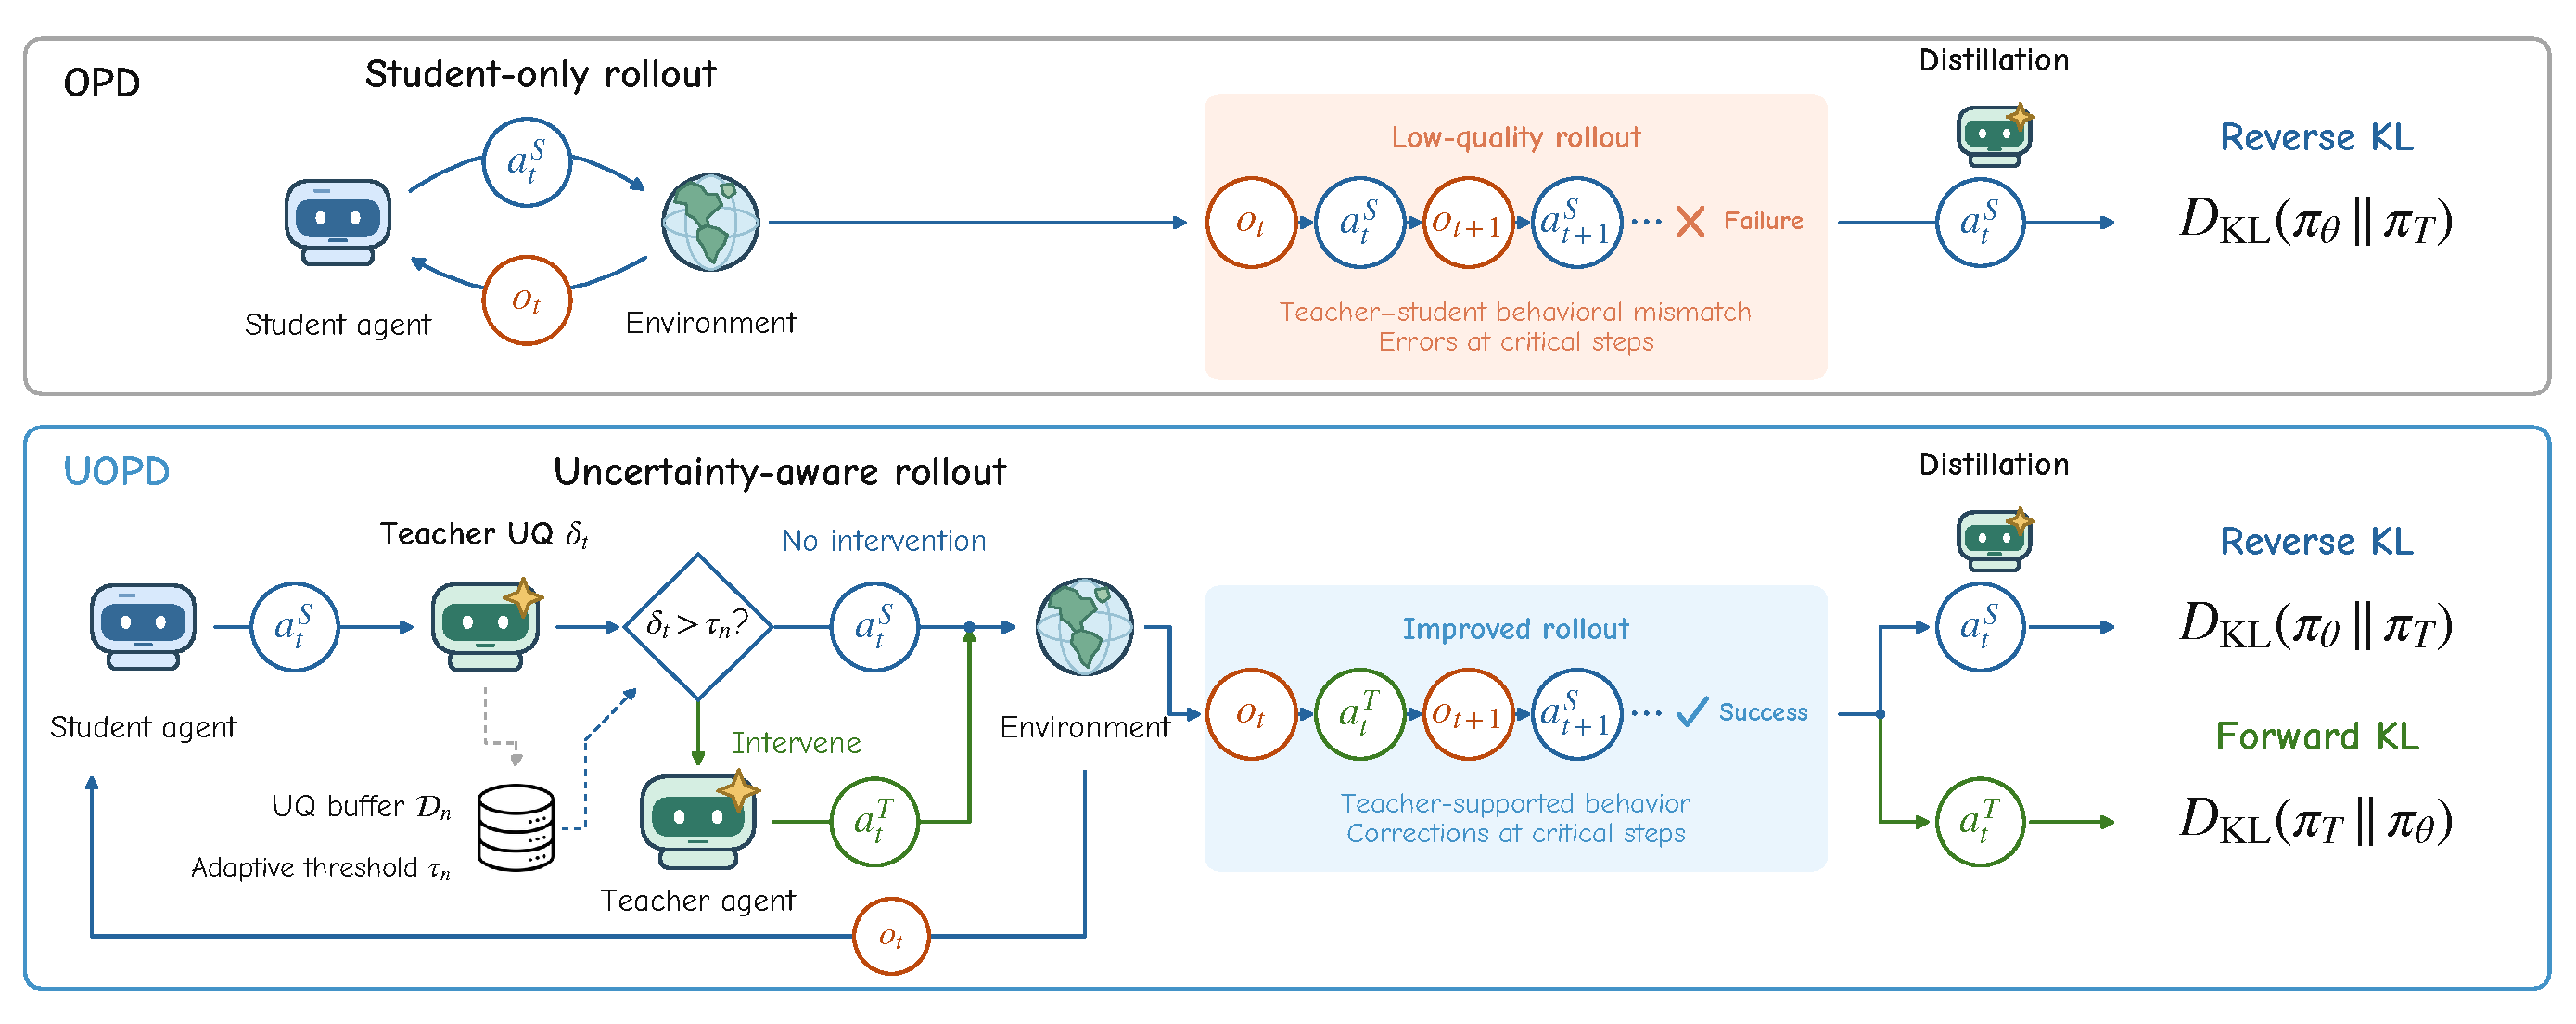
\includegraphics[width=\linewidth]{figures/uai_opd_pipeline.pdf}
\caption{\textbf{OPD versus UOPD.} OPD executes student actions ($a^S_t$) given observations ($o_t$) and distills using reverse KL. UOPD uses teacher signals for uncertainty quantification (UQ) and an adaptive threshold to determine when the teacher intervenes. This decision jointly determines the executed action and the learning objective: reverse KL for student actions, or SFT  on teacher actions ($a^T_t$). The latter minimizes forward KL in expectation.}
\label{fig:opd_comparison}
\vspace{-3mm}
\end{figure}

Distilling a large teacher into a small student has become a standard stage of language-model post-training \citep{hinton2015distilling,agarwal2024policy}. Among its variants, \emph{on-policy distillation} (OPD) has emerged as the dominant recipe: rather than imitating a fixed corpus of teacher trajectories, the student samples its own rollouts and the teacher supplies a dense, token-level target at every state the student actually visits \citep{agarwal2024policy}. This removes the exposure bias of supervised distillation and, by minimizing a reverse Kullback–Leibler (KL) under the student's own distribution, gives the student a mode-seeking target that it has the capacity to match.  Recent work has extended OPD to multi-turn agents, which gather
  information, use tools, and act on successive observations to accomplish
  complex tasks \citep{wang2026exploring,sod2026,sdar2026,sageopd2026}.
  Distilling these capabilities into smaller models is particularly
  valuable for efficient deployment, as completing a single task often
  requires many model calls.

In multi-turn settings, each action shapes subsequent observations and decisions. Student errors can therefore compound across turns, degrading trajectory quality and teacher supervision quality \citep{wang2026exploring,sod2026,manyfaces2026}. Standard OPD can reduce the probability of sampled poor actions through distillation, but does not directly provide better actions for the student to imitate. These poor actions are still executed during rollout collection and can lead to repeated mistakes and task failure. Existing approaches mitigate multi-turn drift by reweighting teacher supervision \citep{sod2026,sageopd2026}, adapting rollout length \citep{pruneopd2026,wang2026exploring}, or using teacher-generated prefixes \citep{wang2026exploring,reopd2026}. However, these approaches do not directly correct unreliable student
  actions at the turns where they arise. Executing such actions can lead
  to further mistakes and task failure, reducing the quality of training
  trajectories. 
  
  To address this gap, we consider \textit{intervention}: replacing selected student actions before execution. As the teacher is generally more capable than the student, it can supply a replacement action for such an intervention, providing explicit corrective targets while guiding the subsequent rollout. We focus on deciding when such intervention is needed. The student may generate actions that elicit high uncertainty from the teacher. This uncertainty offers a potential signal for identifying steps where a teacher correction could be useful.   Our controlled study in Section~\ref{sec:motivation} shows that a single
  teacher correction yields a larger improvement in task success when
  applied at a high-uncertainty turn than at a randomly selected turn.
  These results support using teacher uncertainty to select turns
  for intervention.

Motivated by these findings, we propose \textbf{Uncertainty-Aware Intervention for On-Policy Distillation (UOPD)} (Fig.~\ref{fig:opd_comparison}). At each turn, the student proposes an action, and the teacher evaluates its uncertainty on that action. At low-uncertainty turns, UOPD executes the student action and trains with reverse KL. At high-uncertainty turns, it samples and executes a teacher action and trains the student to imitate it through supervised fine-tuning (SFT), which minimizes forward KL in expectation. Teacher intervention thus supplies an action that the student may rarely generate on its own and lets the student continue interacting from the resulting observation. UOPD uses uncertainty to decide when to learn from the student's own actions and when to introduce a teacher correction.

Our \textbf{contributions} are summarized as follows:

$\bullet$  We propose \textbf{UOPD}, which uses teacher uncertainty to guide
  action execution and supervision in multi-turn on-policy distillation.
  UOPD combines reverse-KL learning on student actions with SFT on executed
  teacher corrections, providing corrective targets and improving
  trajectory quality.\\
$\bullet$ We provide a theoretical analysis of the two roles of teacher corrections.
We derive a rollout return improvement guarantee under average recoverability,
and show that teacher-action imitation can improve student return even when
reverse-KL supervision reduces it.\\
$\bullet$  Experiments on ALFWorld, WebShop, and multi-hop Search demonstrate that UOPD improves task performance over OPD and other state-of-the-art baselines across student model sizes while requiring fewer interaction turns, indicating the effectiveness and efficiency of our method.